\documentclass[12pt]{article}
\usepackage{graphicx}
\usepackage{caption}
\usepackage{subcaption}
\usepackage{verbatim}
\usepackage{url}
\usepackage{listings}
\usepackage[margin=3cm]{geometry}
%\usepackage{titling}
%\setlength{\droptitle}{-12em}

%% Define a new 'leo' style for the package that will use a smaller font.
\makeatletter
\def\url@leostyle{%
\@ifundefined{selectfont}{\def\UrlFont{\sf}}{\def\UrlFont{\small\ttfamily}}}
\makeatother
%% Now actually use the newly defined style.
\urlstyle{leo}


\title{ Private Dropbox \\ Final Report \\ COSC480}
\author{Calum O'Hare \\ Supervisor: David Eyers}
\date{}

\begin{document}
\maketitle

\section{Abstract}
Private decentralised Dropbox. Node to node replication, unison.

\newpage

\tableofcontents
\newpage

\section{Introduction}
\section{Project goal}
The aim of this project is to develop a file synchronisation tool.
Similar to  Dropbox (and others) its main function should be to
keep data synchronised between multiple devices.
What makes it different however is it should:
\begin{itemize}
\item Be decentralised. It will not necessarily need to be run in ``the cloud'' there should be
no centralised server, just many cooperating client nodes. However it should be
possible to configure the system to be centralised if the user wants to. The
system should be flexible in this regard.

\item Allow file synchronisation between multiple clients not just point-to-point
between two clients. Although still synchronise between two Clients as this is the
basis for multiple client synchronisation. Clients may be
running different operating systems. Clients may run on different networks, with different costs of access, including being disconnected from the Internet at times.

\item Allow for fine-grained user control for the majority of the program's
functions, \emph{e.g.}, how often, and what, to replicate within different sets of files. 'What' could be file name, file type, file size, \emph{etc}.

\item Show statistics about which files are being replicated, efficiency (time
taken for the files to become fully up to date),
cost (bandwidth, disk space used). These statistics could also possibly lead
to a heuristic for when to synchronise a given file.

\item Operate automatically, without the user having to initiate a file
synchronisation themselves. The user should be able to set when and
where they would like synchronisation to occur.
\end{itemize}
\section{Background}
There are already many services available
that synchronize your
files. Dropbox, Google Drive, Microsoft SkyDrive, Apple iCloud
all offer cloud based solutions for automatically
synchronizing your files. The problems with these
services is privacy and availability. Storing your data with a
third party gives them access to your documents. If you
are a commercial organisation with sensitive information
this might be concerning. You also cannot guarantee
that you will always be able to access your data, if
the company who owns your data goes bankrupt or
decides to shutdown their service
you could lose all
of your data with little or no warning. 

For example Megaupload.com a file hosting service
has recently been shut down by the United States Department of
Justice for alleged copyright infringement. According to
the founder, 100 million users lost access to 12 billion
unique files\cite{dotcom-trial}.

There are other possible approaches to replicating files
across multiple computers. For example you could use
version control systems like Subversion, Mercurial, and
CVS. One problem with these is that they are
centralised, 
they rely on a central server should that
server fail the replication will break. Not only
that but they create a bottleneck at the server.
Cloud based solutions are also often centralised. 
Another problem is that even if they are decentralised
like git, they won't automatically push updates to other
working sets.

%How about git? It is a distributed tool.
%Auto push updates to other working sets can be done with a few crond scripts

%Add more here?

\subsection*{Example use case}
Here is how I would use such a tool as an example use case.

I like to keep all of the data on my laptop backed up to an
external hard drive. The data on my computer that I wish
to back up falls into three main categories: documents, music, and movies.
Documents are mostly scripts and programs that I am writing for
University or work projects. Documents also include reports for
assessment. These documents change very frequently and are very important
to me. Often these are small files (but not always). My music collection
changes relatively infrequently, files are around $\approx$5MB and I like to
have a relatively current backup of this collection. My movie collection
contains fairly large files but I do not need it to be backed up very often
as it does not change very much and I do not care if I loose a couple of
DVDs. Files that I work on at University would be very useful to have
on my laptop at home. Files that I work on at work mostly stay at work
but occasionally I might want to bring something home to work on.
The other device I always have with me and may be on one of any given
(Wi-Fi or 3G) network at a certain time is my smart phone. I would like
to have photos taken on this backed up to either (or both) my laptop and
external hard drive. 

Some of the files that I move around are of a sensitive or personal nature
and I would prefer not to store them with a third party vendor.
I also have different synchronisation requirements for different
types of data. 
For example my collection of large video files does not change that often
and will chew up valuable network bandwidth whenever it has to transfer
a new file. I like this to be replicated only occasionally as I do not
use it that much. On the other hand my document collection which I use
for work and coursework changes very often, is very important, and
is fairly small. I would like this to be as up to date as possible.

An effective file synchronisation tool would be of
great use to me personally. Dropbox does not do enough
for me. It does not give me enough control over my data.
I want to know which machines my files are going to and when.
I want to feel confident that I will always be able to access
my data even if Dropbox closes down or my internet connection
dies.

%Look at this it is repetitive of above section

\begin{figure}[htp]
    \begin{subfigure}[b]{0.5\textwidth}
        \centering
        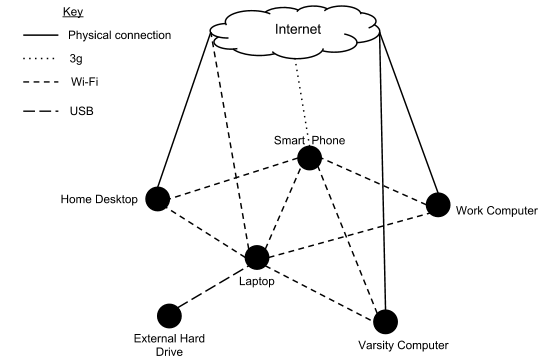
\includegraphics[scale=0.35]{images/PersonalGraph.png}
        \caption{Personal Network}
        \label{fig:personal_graph}
    \end{subfigure}
    \begin{subfigure}[b]{0.5\textwidth}
        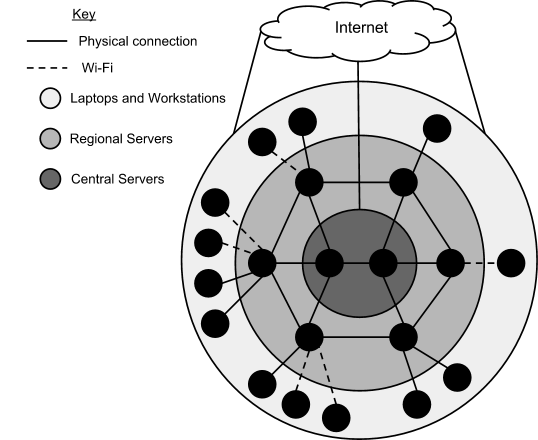
\includegraphics[scale=0.35]{images/CorporateGraph.png}
        \caption{Corporate Network}
        \label{fig:corp_graph}
    \end{subfigure}
\end{figure}

The graph of a personal network has been described above, 
the graph of a  corporate network
is another example use case. It will have many of the same
basic needs as the personal graph. The coloured rings represent
the need for different policies for different machines in a network.
Something which dropbox will not provide but private dropbox will.

% do you need a section to discuss the design of your solution?

\section{Work Done}
I have written a program in python which reads user
settings from a file. Synchronises the appropriate files
to the appropriate machines when they have been modified.
Using an efficient two way file synchronising tool called
unison. I will discuss what I have done and how I have tested
it in this section.

%Update this section
\subsection{Virtual Machines, Node networks}
For testing my program I needed to have a network
of computers that can be linked together in different
arrangements easily. I decided to use virtual machines for
this job since it means I do not need to have a large number
of physical machines.  I can create new machines very easily, and manipulate the
links between them.

I have used Oracle's VirtualBox software. I chose
VirtualBox because of its easy to use command
line interface. I have several scripts that
call the \texttt{vbmoxmange} command to set up the internal
network connections between machines and then start up
the machine itself. This makes switching between
network configurations very easy as I can just
run a different script depending on which network
topology I would like to test.

I have decided to start testing my program with
some simple topologies to see if I can gain any
insight into how best to replicate data around
a network with many nodes. The next step will
be to use those principles and start running
more complicated networks to see how the program
performs.

\begin{figure}[htp]
    \begin{subfigure}[b]{0.5\textwidth}
        \centering
        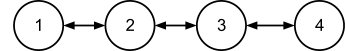
\includegraphics[scale=0.55]{images/line-topo.png}
        \caption{Line topology}
        \label{fig:line_topology}
    \end{subfigure}
    \begin{subfigure}[b]{0.5\textwidth}
        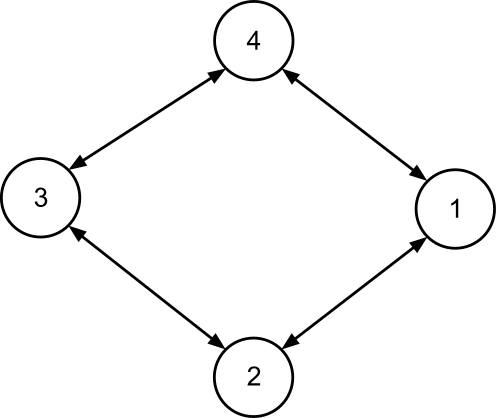
\includegraphics[scale=0.25]{images/circle-topo.png}
        \caption{Circle topology}
        \label{fig:circle_topology}
    \end{subfigure}

    \begin{subfigure}[b]{0.5\textwidth}
        \centering
        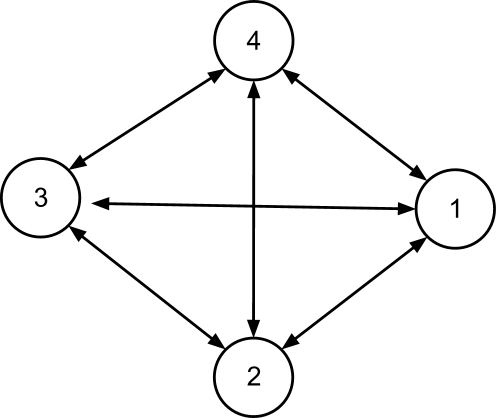
\includegraphics[scale=0.25]{images/con-mesh-topo.png}
        \caption{Connected mesh topology}
        \label{fig:con_mesh_topology}
    \end{subfigure}
    \begin{subfigure}[b]{0.5\textwidth}
        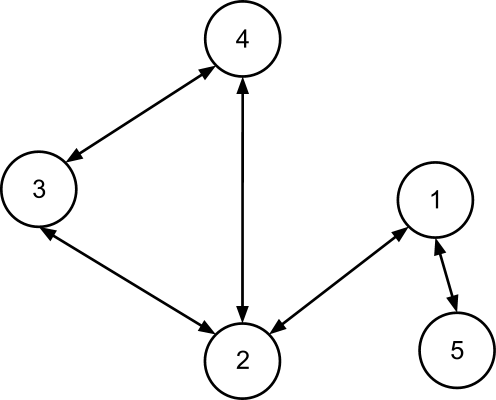
\includegraphics[scale=0.25]{images/other-topo.png}
        \caption{Other topology}
        \label{fig:other_topology}
    \end{subfigure}
    \caption{Simple network topologies}
\end{figure}

Snippet from one of my network scripts:
\begin{verbatim}
VBoxManage modifyvm "Ubuntu-Test" --nic2 intnet
VBoxManage modifyvm "Ubuntu-Test" --intnet2 "intnet"
VBoxManage startvm "Ubuntu-Test"
\end{verbatim}

\subsection{Python}
I have chosen to use Python to implement
my program. Python appealed to me because it
supports many different platforms (Windows, Linux, Mac OS X).
This is useful because it means I will (hopefully)
encounter fewer compatibility problems when running
my program across different operating systems in the future.

%multiproccessing module

\subsection{User control}
One of the main goals of my project is to allow the user
to have a  large amount of control over how the program
behaves. I currently have the program reading from
configuration files that allow the user to specify
which directories they want to watch and where those
directories should be synchronised to.
% give some examples

I chose to use directories as my granularity for replication
as opposed to files because keeping track of a large list
of files may become unwieldy,
% possibly, but you need to be clear what type of unwieldiness you're talking about.
and because I replicate
directories recursively, I can replicate large amounts
of data without a cluttered configuration file.
% this doesn't necessarily follow: your config file could have the ability to include/exclude files and/or directories (possibly recursively). That would give you expressiveness, and still terse config files for many cases.

\subsection{Monitoring Directories}
The application needs to monitor directories for changes
so that it knows when to perform a sync. The reason I have
chosen to do this is because synchronising a directory that
has not been changed is a waste of time and my application
is designed to be as efficient as possible. I do not
however want to be continually polling the watched
directories to see if there have been any changes made.
This would be a significant waste of CPU time. Instead
I have looked into ways of being notified of a
change in the file system below the watched directory.
\begin{itemize}
    \item Inotify
        \begin{itemize}
        \item Inotify is a linux kernel feature that has been
        included in the Linux kernel since version 2.6.
        It is used to watch directories for changes
        and notify listeners when a change occurs. Inotify
        is inode based and replaced dnotify, an older system
        which provided the same function. Dnotify however was
        inefficient, it opened up the file descriptors for
        each directory it was watching which meant the backing
        device could not be unmounted. 
        It also had a poor
        user-space interface which uses SIGIO. Inotify only
        uses one file descriptor and returns events to the
        listener as they occur\cite{inotify-readme}. It works well and does
        what I need it to do. There is a Python module
        called pyinotify that provides a Python interface
        to inotify, which I have used and tested in my program.
        Another reason I chose inotify was because different kinds
        of changes triggered different inotify events. So I
        can differentiate between a file being deleted, created
        or modified \emph{etc}.
        \end{itemize}

    \item FSEvents
        \begin{itemize}
        \item FSEvents is an API in MacOS X\cite{fsevents-intro}. It is similar
        to inotify in that it provides a notification to other
        applications when a directory is changed however
        it does not inform you which file in the directory
        was changed. This does not matter for my
        application since Unison is smart enough not to copy
        unchanged files in a directory. There is a Python module
        for FSEvents, as well. 
        
        I also looked at using the \texttt{kqueue}\cite{kqueue-man} system call that is
        supported by OS X and FreeBSD. It notifies the user
        when a kernel event occurs. I decided against using
        \texttt{kqueue} as the high level approach of FSEvents,
        suits the application's needs.
        \end{itemize}

    %\begin{comment}
    \item ReadDirectoryChangesW
        \begin{itemize}
        \item Windows, like the other operating systems
        I have looked up, provides a nice way of doing this
        too. There is a function called ReadDirectoryChangesW.
% you're not implementing ReaddirectoryChangesW - rephrase?
        There is a FileSystemWatcher Class in .NET version 4 and
        above. IronPython might prove to be a good choice for a
        Windows implementation. I have chosen only to implement
        my program on linux because portability wasn't in the main
        scope of the project. It would have been nice to look
        at it further but became too time consuming.
% perhaps clarify why you think it wold be appropriate if you still have more to learn about it.
        \end{itemize}
    %\end{comment}
\end{itemize}

\subsection{Point-to-Point synchronisation}
After some preliminary analysis of the available file synchronisation
tools I have found a tool called Unison to be a promising starting
base for this project. Unison is an open source file synchronisation tool.
It supports efficient (\emph{i.e.,} it attempts to only send changes between file versions) file synchronisation between two
directories (including sub-folders) between two machines (or the same
machine).

I decided to run some tests using unison 
and the network
I had set up to determine whether this would make a good base for
my program or not.

I looked at three methods of file synchronisation across
different networks. Naive copying; using rsync, an application
designed for efficiently copying files in one direction by looking at
the differences in the files; and unison described above.

\begin{figure}[htp]
    \centering
    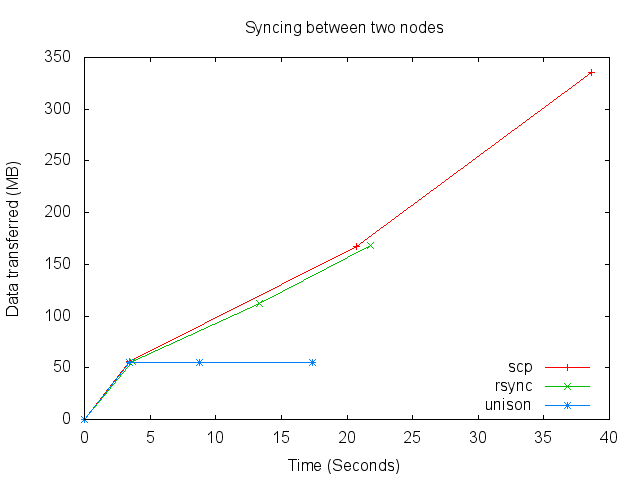
\includegraphics[scale=0.5]{images/two-point-comp-same.png}
    \caption{Comparison of scp,rsync,unison}
    \label{fig:point_comp_graph}
\end{figure}

Rsync and unison performed significantly better
than the naive copy method (as expected). After the initial file
transfer subsequent edits to the file meant much less data had to
be transmitted over the network, which meant the node graph
became up to date much more quickly.

The reason naive copy sent over 300Mb of data to copy three 50Mb
files was because my implementation is deliberately naive, it will
copy the entire directory each time it is changed. For rsync and
unison this is not a problem because they work based on the
differences between the files. However copy doesn't look at
the files it just copies everything in the directory tree.
Hence it will copy 50Mb after file one is created, 100Mb after
the second file is added and finally 150Mb when all three
files are present.

50Mb + 100Mb + 150Mb = 300Mb

Rsync copies the expected 150Mb for three 50Mb files. While
Figure \ref{fig:point_comp_graph} illustrates another advantage
of unison over rysnc. The graph shows three zero filled
binary files being copied from one node to another one after
the other. Unison recognised that even though the files were named
differently they were the same file. Another advantage of unison
is that it handles replication in two directions without
clobbering the files on the other side.

Each of the three methods I trialled had some overhead associated
with them. This overhead was due to the ssh tunnel between the
machines which all three methods used. Unison and rsync also
require some overhead when checking the differences between the files
in the directories. This is why the graph shows the three lines
slightly above where you might expect them to be for the amount
of data that was copied.

\section{Full graph replication}
\begin{figure}[htp]
    \begin{subfigure}[b]{0.5\textwidth}
        \centering
        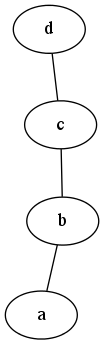
\includegraphics[scale=0.4]{images/line-graph.png}
        \caption{Line - Generated Graph of Topology}
        \label{fig:line_graph}
    \end{subfigure}
    \begin{subfigure}[b]{0.4\textwidth}
        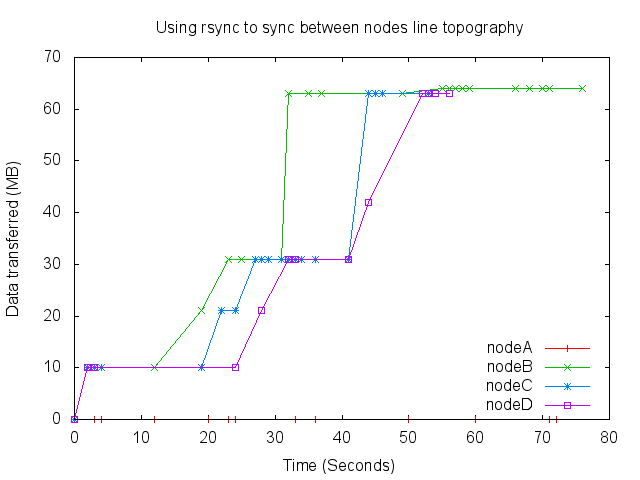
\includegraphics[scale=0.4]{images/line-scp-wrong.png}
        \caption{SCP}
        \label{fig:line_scp}
    \end{subfigure}

    \begin{subfigure}[b]{0.75\textwidth}
        \centering
        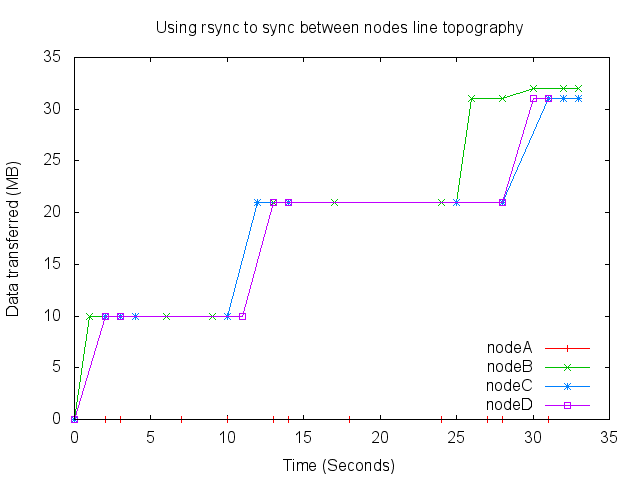
\includegraphics[scale=0.4]{images/line-rsync.png}
        \caption{Rsync}
        \label{fig:line_rsync}
    \end{subfigure}
    \begin{subfigure}[b]{0.4\textwidth}
        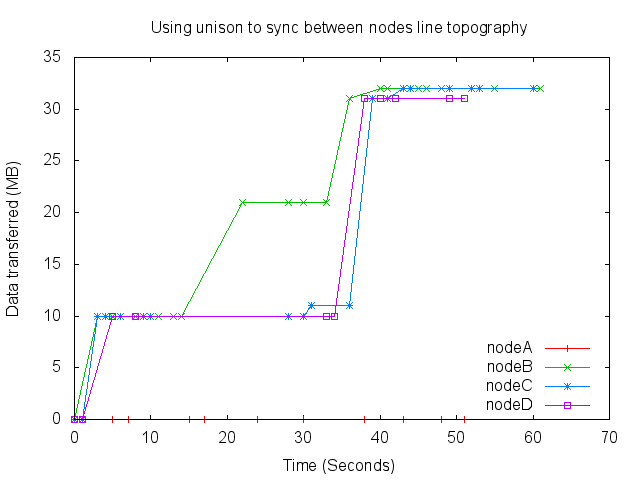
\includegraphics[scale=0.4]{images/line-uni.png}
        \caption{Unison}
        \label{fig:line_uni}
    \end{subfigure}
    \caption{Comparison of methods over line topology}
\end{figure}

\section{When to stop copying}
After testing my program on some simple topologies one problem became
clear. Each node would notice changes had occurred to a folder
it was watching and would then try to copy these changes to other
nodes that it was connected to. The problem was that if the changes
came from one of its neighbour nodes this would cause an infinite loop
of two nodes trying to copy changes to each other. This was particularly 
a problem when using scp to copy. When using Unison this was not as much of
a problem because it could detect that no changes had occur between the nodes
and would stop syncing after one check (which had minimal overhead).

\begin{figure}[htp]
    \centering
    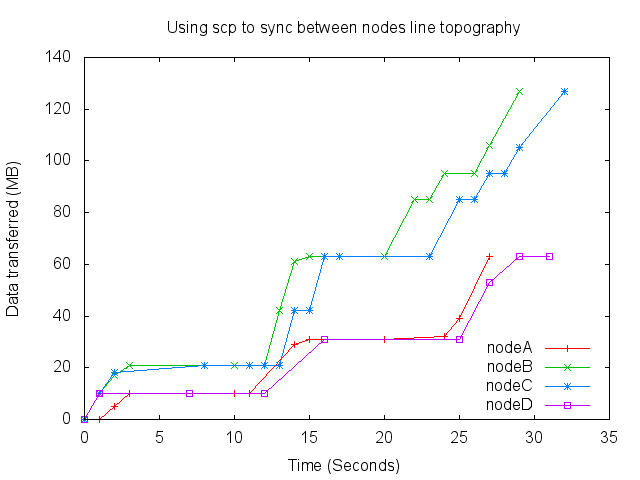
\includegraphics[scale=0.5]{images/line-scp-back.png}
    \caption{Line topology, using scp, nodes copying data back and forth}
    \label{fig:line_scp_back_forth_graph}
\end{figure}

\begin{figure}[htp]
    \centering
    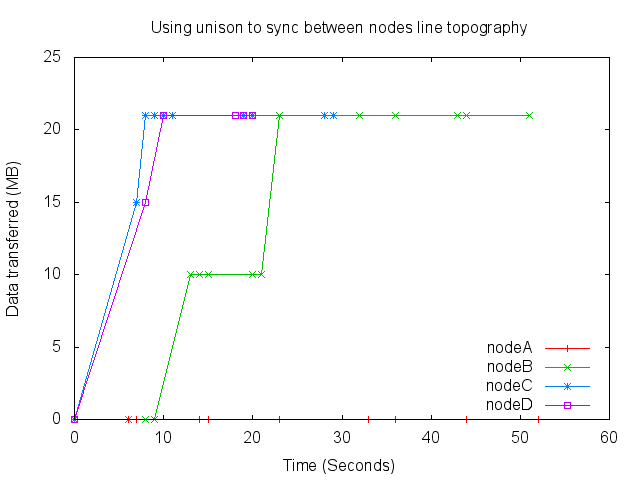
\includegraphics[scale=0.5]{images/line-uni-10-tail.png}
    \caption{Line topology, using unison, unnecessary checking}
    \label{fig:line_uni_tail_graph}
\end{figure}

Figure \ref{fig:line_scp_back_forth_graph} shows three 10Mb files being copied to a node
in a line topology. The problem is that nodeB and nodeC continue to send
data to each other even after every node has all of the files. NodeA receives
a lot of data even though it was the source of the file changes. 

The data points in figure \ref{fig:line_uni_tail_graph} show that when using
unison although no extra data was sent unison had to make checks to see
whether there were any changes or not.

%Change this
I used a configuration file to get around this problem. Each time a node
synchronised with another node it would write out a configuration file telling
the other node what files had been copied, who sent them and what the
modification time of the files were. In this way a node could check
if it was about to synchronise a file back to the node it received
the file from or if it had local changes that were newer than a received
file it could continue with its sync.

\section{Sub-nodes}
I chose to classify directories as 'sub nodes' of a graph. The reason I choose
directories is because they are easy to manage a configuration file of directories to
keep in sync (from the users point of view). If we wanted to only synchronize
certain files in a directory we could write a unison configuration file with 
exclusions/inclusions in it. The other reason directories are a good choice
is because I can have different directories in different places on different
file systems by using symbolic links. I wanted to see how the freshness of different
sub-nodes varied between nodes when the program was running.

\begin{figure}[htp]
    \centering
    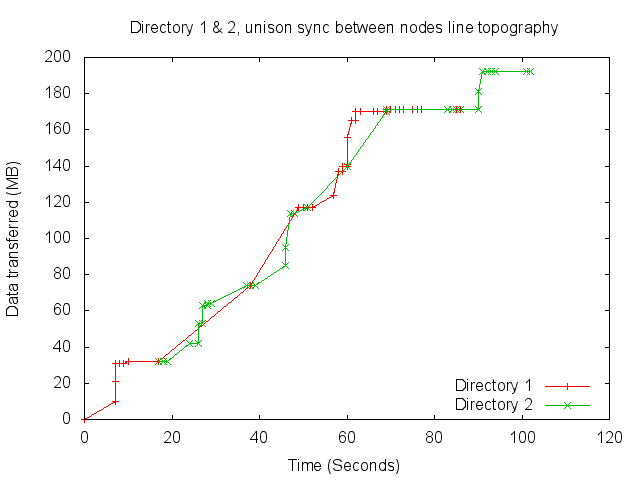
\includegraphics[scale=0.5]{images/line-uni-2dir-comb.png}
    \caption{Line topology, using unison, two different directories being synced}
    \label{fig:line_uni_2dir_comb_graph}
\end{figure}

\section{How often to sync}
So how often should I sync once I noticed a change.
If lots of small changes are occurring frequently it might be more efficient
to perform a synchronisation after several changes have occurred. Given that
there is overhead with each synchronisation, fewer copies means less data
sent over the network.

\section{Unison and temporary files}
I noticed that when Unison ran it created temporary files in the
directory and once these files had been fully copied it renamed
them to their intended name. The problem with this was that my program
was picking up these temporary files as they were created and trying to
copy them to the next node, only to find that these files no longer existed.
To get around this problem I decided to implement a filter on the files to
be copied. The program filters out files that contain ".tmp" in the filename.
Unison is not the only program that uses temporary files. I decided that this
should be a user set preference given that users may want to filter out different
files.

My program simply reads from a file with each file pattern to exclude
listed on a new line. It is easy to add to/remove from. As I said above
I added .tmp to the file as a default. This could easily be extended
to allow a user to omit certain files from the replication by adding
all files in my programs ignore file to unisons ignore list. Or conversely
by maintaining a white list of files to sync. This would allow for
greater granularity when syncing nodes.

\section{Future work}
\subsection{Full node graph replication}
I am going to be looking into the most efficient way to
replicate data between many nodes in a graph, where nodes are machines
running the program and edges in the graph are connections
between machines such as over Wi-Fi, USB, or through the internet, \emph{etc}.
Each connection may have different properties associated
with it, for example each link may have a different cost
associated. The two costs that I am most interested in
are data throughput and latency. There may be data caps to worry about
(for 3G especially) or costs associated with usage
(this could be money charged per megabyte used or
the time cost of sending a lot of data over an (potentially)
already busy/important channel). The link may be down
temporarily or may rarely be up. The task here will be
to find algorithms that give as near to optimal as possible,
given certain conditions and preferences,
to shift data between all the necessary nodes
efficiently and with minimal cost. 
Cost will most likely involve keeping the number
of bytes passed over the network(s) to a minimum.
Efficiency will depend on personal preference and
the situation, ideally one would not want to have
to be waiting on replication to occur but this
should not come at the expense of extreme cost, however.
There will be an infinite number of use cases for this
project which means an infinite number of graphs,
however I will attempt to look at common use cases
and as many different types of graph as possible.

\subsection{Sub-Nodes}

The other aspect of the ``multiple nodes in the graph'' problem
is that each node will most likely be made up of many smaller nodes.
Each user will be unlikely to select the root directory of the
file system to synchronise, which means they may select a few
different directories on the file system. This gives us ‘sub nodes’
that the main node is still the machine as above. The sub nodes are
an individual directory or set of directories that are set to be replicated.
The reason this is interesting is because each of these ‘sub nodes’
may have different synchronisation settings (see fine-grained controls).
This leaves us with the possibility of machines being fully up to date,
partially up to date, or completely out of date with all other nodes in
the graph. 

An example of this potential situation is shown below.
This sort of graph ties in with the statistics/feedback side of the
project. How out of date is the graph at any given time?
If the graph contains out of date data, do we ever expect it
to get back  to being completely up to date? How long do we expect
this to take? How do these facts reflect on the synchronisation settings
we chose? Can we improve on the ‘performance’ by tweaking the settings?

%Insert sub node image
\begin{figure}[htp]
    \centering
    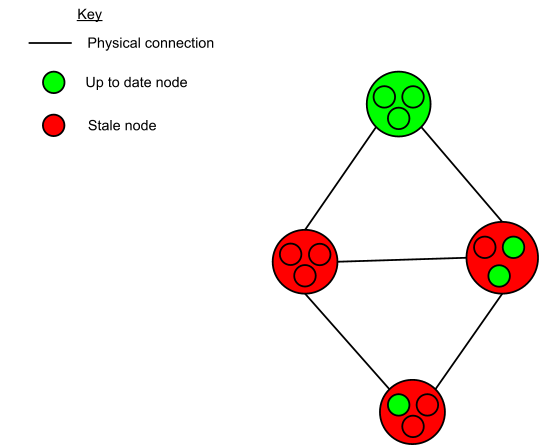
\includegraphics[scale=0.5]{images/sub-node.png}
    \caption{Graph of sub nodes within nodes}
    \label{fig:sub_node}
\end{figure}

\newpage
\subsection{Mobile nodes}

Connections between nodes in the graph (edges) may
change over time. This could be because one of the nodes
is a laptop and joins different networks at different
times or because a network/machine is unreliable and is
not up at a given point in time. I have represented
edges that behave in this way as grey on the diagram below.
I will refer to nodes with grey edges as `mobile' nodes.

It will be interesting to see how mobile nodes affect how
up to date the nodes in the graph are. We might expect that
nodes that are not available for very long periods lag behind
others that are. We might also expect that if a mobile
node is a link between two parts of the network that
these two parts fall out of synchronisation. I want to look
at how nodes in the graph may get smarter about how
they use unreliable edges. I will do this by having
the edges up or down at different points in time
and taking snapshots of the graph as it is at that time.

%Insert mobile node image
\begin{figure}[htp]
    \centering
    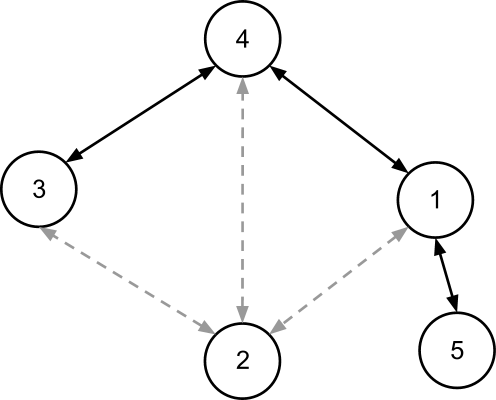
\includegraphics[scale=0.5]{images/mobile-node.png}
    \caption{Node two moves within the graph}
    \label{fig:mobile_node}
\end{figure}

In figure \ref{fig:mobile_node} node two intermittently has a 
connection to a subset of
nodes 1,3 and 4. The edges in grey are links that
are not always present.

\newpage
\subsection{More user control}

Due to the highly unpredictable nature of the graph the user
should be able to greatly affect how the program runs.
A user should be able to set how often replication occurs and
under what conditions it should occur \emph{e.g.} only when
connected to a certain network.

For example replicate
‘my documents’ \texttt{/Users/Calum/Documents} on my laptop every hour to
work but only when connected to the work Wi-Fi network.
There should be some intelligent indication of how certain options
may affect performance which relates to the next section. This
may be able to be estimated by looking at previous running settings
and seeing what effect they had on the network. This ties in with the
next section.

\subsection{Feedback}
% OK - I'm assuming this is into mental notes rather than proposed text. Overall, I think it wold be good for you to overview and justify your high-level plan, as well as the more detailed aspects.

Private dropbox should keep logs of what is happening with
the system at the current point in time. 
It should log:
\begin{itemize}
    \item what the current user settings are.
    \item how much data is being transferred between the nodes.
    \item which links between nodes are being used the most.
    \item how up to date each part of the graph is.
\end{itemize}

I will then look at presenting this information
in a meaningful way to the user.
One way to do this would be when the user changes the
settings. Private dropbox could then estimate whether that
change will speed up or slow down overall synchronisation
of the graph and pass that (potentially) useful information
to the user.

\section{Results}

\section{Conclusion}


\begin{thebibliography}{9}

\bibitem{dotcom-trial}
Foreman, Michael "Kim Dotcom v United States of America". Computerworld. 3 February 2012.

\bibitem{inotify-readme}
www.kernel.org/pub/linux/kernel/people/rml/inotify/README, 22 September 2004.

\bibitem{fsevents-intro}
Apple Inc. \url{https://developer.apple.com/library/mac/#documentation/Darwin/Conceptual/FSEvents_ProgGuide/Introduction/Introduction.html}, 11 October 2011.

\bibitem{kqueue-man}
Apple Inc. \url{http://developer.apple.com/library/mac/#documentation/Darwin/Reference/ManPages/man2/kqueue.2.html}

\end{thebibliography}

\section{Bibliography}
%OPTIONAL: further reading

\section{Glossary}
%OPTIONAL

\section{Index}
%OPTIONAL

\section{Appendices}
%OPTIONAL


\begin{figure}[htp]
    \centering
    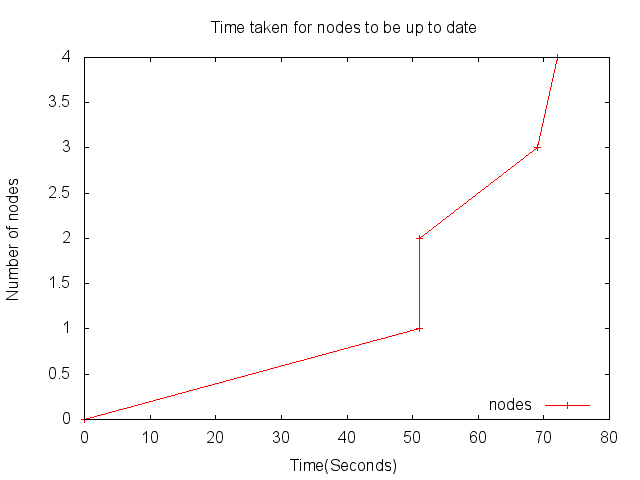
\includegraphics[scale=0.5]{images/fintime.png}
    \caption{Unison, line, finishing times}
    \label{fig:fintime_graph}
\end{figure}


\begin{figure}[htp]
    \centering
    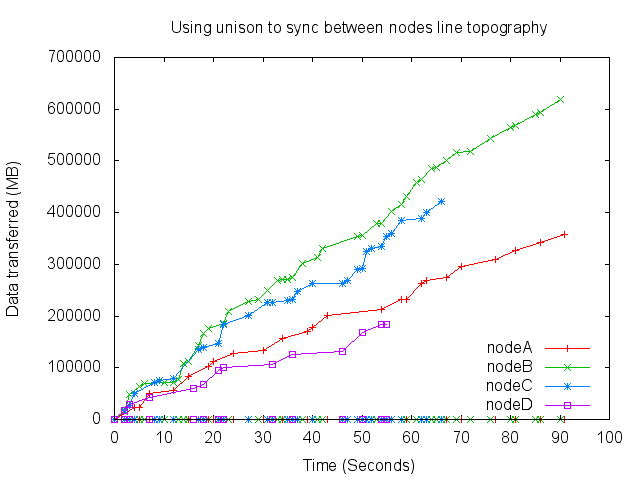
\includegraphics[scale=0.5]{images/rand-txt-2sleep.png}
    \caption{2 seconds sleep text file}
    \label{fig:2sleep_graph}
\end{figure}

\begin{figure}[htp]
    \centering
    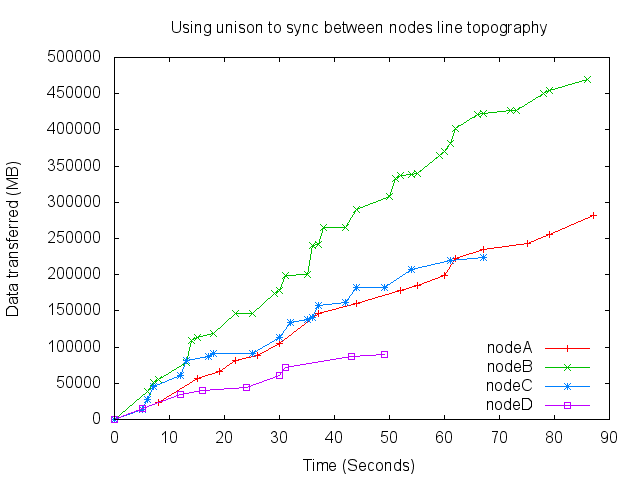
\includegraphics[scale=0.5]{images/5sleep-bad.png}
    \caption{5 seconds sleep text file}
    \label{fig:5sleep_graph}
\end{figure}

\newpage
WatchAndSync.py
\lstinputlisting{code/watchandsync.py}

\newpage
ReadNet.py
\lstinputlisting{code/readnet.py}

\newpage
onTheFly.sh
\lstinputlisting{code/onTheFly.sh}

\end{document}
